%%
%% Copyright 2007, 2008, 2009 Elsevier Ltd
%%
%% This file is part of the 'Elsarticle Bundle'.
%% ---------------------------------------------
%%
%% It may be distributed under the conditions of the LaTeX Project Public
%% License, either version 1.2 of this license or (at your option) any
%% later version.  The latest version of this license is in
%%    http://www.latex-project.org/lppl.txt
%% and version 1.2 or later is part of all distributions of LaTeX
%% version 1999/12/01 or later.
%%
%% The list of all files belonging to the 'Elsarticle Bundle' is
%% given in the file `manifest.txt'.
%%

%% Template article for Elsevier's document class `elsarticle'
%% with numbered style bibliographic references
%% SP 2008/03/01
%%
%%
%%
%% $Id: elsarticle-template-num.tex 4 2009-10-24 08:22:58Z rishi $
%%
%%
\documentclass[preprint,12pt,3p]{elsarticle}

%% Use the option review to obtain double line spacing
%% \documentclass[preprint,review,12pt]{elsarticle}

%% Use the options 1p,twocolumn; 3p; 3p,twocolumn; 5p; or 5p,twocolumn
%% for a journal layout:
%% \documentclass[final,1p,times]{elsarticle}
%% \documentclass[final,1p,times,twocolumn]{elsarticle}
%% \documentclass[final,3p,times]{elsarticle}
%% \documentclass[final,3p,times,twocolumn]{elsarticle}
%% \documentclass[final,5p,times]{elsarticle}
%% \documentclass[final,5p,times,twocolumn]{elsarticle}

%% if you use PostScript figures in your article
%% use the graphics package for simple commands
%% \usepackage{graphics}
%% or use the graphicx package for more complicated commands
%% \usepackage{graphicx}
%% or use the epsfig package if you prefer to use the old commands
%% \usepackage{epsfig}

%% The amssymb package provides various useful mathematical symbols
\usepackage{amssymb}
\usepackage[spanish]{babel}
%% The amsthm package provides extended theorem environments
%% \usepackage{amsthm}

%% The lineno packages adds line numbers. Start line numbering with
%% \begin{linenumbers}, end it with \end{linenumbers}. Or switch it on
%% for the whole article with \linenumbers after \end{frontmatter}.
%% \usepackage{lineno}

%% natbib.sty is loaded by default. However, natbib options can be
%% provided with \biboptions{...} command. Following options are
%% valid:

%%   round  -  round parentheses are used (default)
%%   square -  square brackets are used   [option]
%%   curly  -  curly braces are used      {option}
%%   angle  -  angle brackets are used    <option>
%%   semicolon  -  multiple citations separated by semi-colon
%%   colon  - same as semicolon, an earlier confusion
%%   comma  -  separated by comma
%%   numbers-  selects numerical citations
%%   super  -  numerical citations as superscripts
%%   sort   -  sorts multiple citations according to order in ref. list
%%   sort&compress   -  like sort, but also compresses numerical citations
%%   compress - compresses without sorting
%%
%% \biboptions{comma,round}

% \biboptions{}


\journal{Nuclear Physics B}

\begin{document}

\begin{frontmatter}

\title{Retos de la inteligencia artificial para el desarrollo sostenible en el Ecuador¨. {Challenges of artificial intelligence for sustainable development in Ecuador}\tnoteref{label0}}
\tnotetext[label0]{Este es el resultado del trabajo grupal para la escritura de un artículo}


\author[label1,label4]{Diana Romero Córdova\corref{cor1}\fnref{label3}}
\address[label1]{Universidad Internacional de la Rioja}
\address[label4]{Universidad Católica de Cuenca\fnref{label4}}

\cortext[cor1]{Los tres somos los autores de este artículo}
\fntext[label3]{Informo que esta es una plantilla de latex descargada con el formato de elseiver para redacción de artículos.}
%%\fntext[label4]{Small city}

\ead{diromeroc@hotmail.com}
\ead[url]{iasostenible.com}

\author[label1,label5]{Santiago Luna Romero}
\address[label5]{Universidad Politécnica Salesiana}
\ead{sanfeluro@gmail.com}

\author[label1,label5]{Daniel Proaño Guevara}
\ead{daniel.p.ecu@ieee.org}

\begin{abstract}
El presente artículo es un resumen de la investigación que se efectuó como parte de un estudio sobre los objetivos del desarrollo sostenible. Varios son los desafios que enfrentan los gobiernos para garantizar su cumplimiento. En el Ecuador cada día se enfrentan nuevos y numerosos retos tecnológicos para mantener la competitividad que va acompañado de la necesidad de mantener un desarrollo sostenible. La inteligencia artificial abre un abanico de oportunidades de desarrollo pero es importante mencionar los ejes que permitirán garantizar la conservación del medio ambiente y la vida de las futuras generaciones. El método empleado fue de revisión bibliográfica, no tiene intervención, es transversal y descriptivo, permite identificar los aspectos a considerar en el uso de la inteligencia artificial para cumplir los objetivos propuestos en el plan nacional toda una vida.
\end{abstract}

\begin{keyword}
%% keywords here, in the form: keyword \sep keyword
inteligencia artificial, desarrollo sostenible, retos.
%% MSC codes here, in the form: \MSC code \sep code
%% or \MSC[2008] code \sep code (2000 is the default)
\end{keyword}

\end{frontmatter}

%%
%% Start line numbering here if you want
%%
% \linenumbers

%% main text
\section{Introducción}
\label{sec1}
Hoy más que nunca estamos conscientes de las necesidades ambientales de todo el planeta tierra. No es únicamente tarea de los gobiernos desarrollar estrategias que garanticen el mantenimiento del medio ambiente, también es responsabilidad de sus habitantes y de las diferentes instituciones, aunque contradictoriamente también es una prioridad mantenerse altamente competitivos. El avance tecnológico optimiza diferentes procesos para el desarrollo de los pueblos aunque en ocasiones eso implica contribuir a un desgaste ambiental.\\

Alrededor del término desarrollo sostenible se han generado planes, programas y estrategias enfocados en la satisfacción de las necesidades de las generaciones del presente sin limitar la satisfacción de las necesidades de las generaciones futuras. Este trabajo analiza los ejes de la inteligencia artificial para lograr el objetivo mundial de la conservación.\\

Este trabajo tiene usa sección del estado del arte, donde se pueden identificar los avances de la inteligencia artificial en el mundo entero en cuanto a los objetivos del desarrollo sostenible, en el siguiente apartado se detallan los materiales y métodos utilizados para desarrollar esta investigación seleccionando intencionalmente los documentos propuestos por el gobierno nacional para su estudio. \\

En el apartado de resultados, se hace un desglose de cada uno de los ejes de los objetivos de desarrollo, para identificar la necesidad en algunos de los aspectos, de la intervención de técnicas de inteligencia artificial para asistir y facilitar su cumplimiento. Finalmente en las conclusiones se describen los puntos más importantes que el gobierno nacional debe empezar a impulsar para lograr la consecución de los objetivos en el corto plazo.


\section{Estado del arte}
\label{sec2}
En el Ecuador cada día se introducen nuevas tecnologías que permiten la consecución de objetivos en cuanto a la productividad, formación profesional, inversiones, finanzas, salud, entre otras. También hace uso de las aplicaciones inteligentes como Siri de Apple, Alexa de Google, entre otras, que a la vez inducen a la generación de nuevas ideas de desarrollo tecnológico basado en inteligencia artificial. \\

La energía eléctria por ejemplo, es una muestra de que en Ecuador se han gestionado mejor los recursos energéticos, promoviendo la proteccion del medio ambiente y con cumplimiento estricto de normas de calidad y servicio. Las llamadas Smart Grids, centraliza el uso de la información para el beneficio de los usuarios mejorando el servicio del sistema eléctrico. Se potencian la eficiencia energética además de una gestión de la energía oportuna.\cite{alava2016aplicacion} \\

De igual manera en la Escuela Politécnica del Chimborazo, se utiliza la inteligencia artificial para realizar el monitoreo de la red eléctrica del laboratorio de máquinas. \cite{coronel2017monitoreo}\\

Otros estudios en el Ecuador han llevado a desarrollar por ejemplo un brazo robot para el reconomiento y manipulación de objetos, controlado por inteligencia artificial \cite{de2014brazo}, lo que ha permitido beneficiar a personas de escasos recursos económicos para sobrellevar la pérdida de una de sus extremidades, esto como resultado del programa de ayuda a personas afectadas por explosiones mineras.\\

La salud será beneficiaria desde sensores inteligentes que controlan el azúcar en la sangre entre otros aspectos. Actualmente el uso de smartwatches permiten controlar la salud de manera individual y voluntaria a su usuario. Con las técnicas de redes neuronales se controla y predice una posible elevación del índice de la presión arterial de las personas. Con el uso de estas tecnologías y vinculado a la telemedicina, se controla la salud de los pacientes en riesgo desde los hospitales más cercanos. \cite{ledo2019inteligencia}\\

La construcción de viviendas en beneficio de las personas adultos mayores, mujeres y niños de escasos recursos que viene desarrollando el Ministerio de Desarrollo Urbano y de Vivienda, se ha apoyado en un sistema para pronosticar el comportamiento de construcción de viviendas en el país a través del tiempo con el uso de técnicas de inteligencia artificial \cite{delgado2007sistema}\\

El estudio de la ética para los ámbitos de la vida en el Ecuador, también han sido discutidos. La actualización de la ley con referencia a los diferentes usos de los datos que son la huella de las diferentes actividades que se realizan en espacios virtuales, de consulta en las redes de internet, el intercambio en redes sociales, las compras y las búsquedas, que permiten identificar los gustos y preferencias de los usuarios. También es un reto para el desarrollo controlar el uso de la inteligencia artificial en estos términos. \cite{rodriguez2019modelo}\\

En la educación el uso de micromundos lúdicos interactivos permiten una interacción de los niños con objetos dotados de inteligencia, de tal forma que no solo se desarrollen los aprendizajes motores y colaborativos, sino además se pueden identificar los comportamientos psicológicos que permitan una intervención temprana. \cite{cayambe2016inteligencia}\\

Los controles de velocidad de los automóviles tambien se realizan con técnicas de inteligencia artificial. En Ecuador se ha desarrollado un algoritmo de inferencia difuso para controlar la velocidad y detectar los obstáculos que se presentan en el camino y evitar que el automóvil choque cuando el conductor sufre cualquier alteración de su cuerpo, el prototipo recoge información de su entorno para la toma de decisiones, la simulación está hecha en Matlab y la experimentación en tiempo real con Arduino empleando java como interfaz. \cite{mejia2019control}\\

Los objetivos del desarrollo sostenible impulsan a buscar y desarrollar cada día tecnología más avanzada para el beneficio de la humanidad, razón por la que el termino de inteligencia artificial responsable IAR se erige para dar cumplimiento a las exigencias de la agenda 2030.\cite{rodriguez2019modelo} acompañado de un cambio en la cultura de generación de conocimiento innovador.\\

El ecosistema tecnológico permite resolver con mayor facilidad los problemas de la vida cotidiana como de empresas y organizaciones. Está conformado principalmente por el desarrollo de las áreas de la inteligencia artificial, la robótica, el internet de las cosas, la biotecnología entre otras \cite{pinillos2019pasado}\\

Varios estudios sobre las diferentes técnicas de inteligencia artificial y su aplicación en la conservación del ambiente permiten mantener un panorama optimista en cuanto al desarrollo de propuestas para el cuidado y protección de los aspectos más vulnerables y prioritarios, como lo demuestra la investigación realizada con el uso de la minería de texto y el aprendizaje automático que permiten destacar la importancia del cuidado de la seguridad, educación y calidad de vida del pueblo colombiano \cite{gomez2019mineria}.\\

Las Smart Cities pueden ser la respuesta a ciudades más eficientes y sostenibles. Aplican nuevas tecnologías para la mejora de la calidad de vida de las personas asegurando un desarrollo económico, social, ambiental y sostenible. Para ello es importante el estudio y desarrollo de aplicaciones y prototipos que solucionen los principales problemas de la sociedad y el entorno \cite{villagra2019hacia}.\\ 

El área del turismo de también es uno de los objetivos de los gobiernos, la promoción y difusión de las áreas con belleza natural, con historia y modernismo deben atraer a propios y extraños para disfrutarla. La información de los turistas nacionales y extranjeros deja huella en redes sociales, navegadores y páginas de intercambio de información, es a través de ellas que se puede extraer información sobre las necesidades, los gustos, su comportamiento en el viaje y sus consumos y pagos. Para cada turista se puede crear una recomendación de acuerdo a sus gustos, con el uso del procesamiento del lenguaje natural y el aprendizaje automático.\cite{almeida2019robots}\\

La lucha contra la pobreza con el uso de la inteligencia artificial logrará llegar a la población que realmente lo necesitan, será posible la caracterización de los sectores subnormales en base a datos proporcionados por la población más vulnerable.\cite{arroyave2019inteligencia} 
Según Houlin Zhao, Secretario General de la UIT, "la inteligencia artificial  sigue evolucionando con rapidez… y tiene un enorme potencial para el bien social." \\ 

La educación forma parte de los objetivos del plan de desarrollo, con el uso de la inteligencia artificial en ámbitos de formación, la educación a a distancia posibilita el aprovechamiento del conocimiento del alumno, puesto que incorpora nuevas tecnologías como tutores inteligentes que ayudan a los alumnos en momentos que se ven confundidos y no avanzan con el estudio de los temas. \cite{vila2007monografia}\\

En el área de la salud la inteligencia artificial viene creciendo a pasos agigantados, la detección con algoritmos de reconocimiento de patrones en muestras como el ADN facilitan la detección temprana de enfermedades como el cáncer, también se estan usando en imágenes diagnósticas para prevenir infartos por ejemplo. \cite{arroyave2019inteligencia}, al entrenar un algoritmos de aprendizaje automático con todas las imágenes generadas en procesos de exploración en RX, es fácil predecir padecimientos posteriores en los pacientes que afecten a su salud. \\

``Las nuevas tecnologías pueden beneficiar las vidas de muchas personas alrededor del mundo. Por ejemplo, pueden mejorar la seguridad alimentaria, reducir los desperdicios y ayudar a las economías locales a crecer a través del acceso a nuevos mercados y formas de financiación", declaró Amina Mohammed durante la reunión celebrada en la sala del ECOSOC.\\

David Hanson, el creador de Sophia, una robot inteligente desarrollada por la compañía Hanson Robotics, menciona que Sophia que es capaz de interactuar con humanos, hablar, responder preguntas e incluso hacer gestos, mencionó que la inteligencia artificial puede crear máquinas que son inteligentes y adaptativas, que pueden hacer del planeta un mejor lugar para las personas.

\section{Materiales y métodos}
\label{sec4}
Para encontrar los beneficios y usos actuales de la inteligencia artificial frente al los objetivos del desarrollo sostenible, esta investigación analizó el proyecto "Ecuador 2030 productivo y sostenible", promovido por el Comité Empresarial Ecuatoriano, el cual incluye a más de 80 organizaciones gremiales nacionales de todos los sectores: agrícola, construcción, turismo, industrial, comercial y financiero.\\

El proyecto posee tres objetivos principales: que las empresas respondan de forma adecuada a los retos tecnológicos de la Cuarta Revolución Industrial, que las empresas definan y adopten modelos de negocios disruptivos para crecer de forma exponencial, y, que las empresas incorporen criterios de sostenibilidad en sus modelos de negocio, alineándose con los Objetivos del Desarrollo Sostenible.\\

A su vez se realizó la constatación de la alineación de los objetivos del proyecto mencionado anteriormente con el plan nacional de desarrollo "Toda una Vida" del Gobierno de la República del Ecuador.
En el análisis de los documentos que buscan el desarrollo sostenible, cabe destacar la importancia que se otorga al uso de la tecnología en el adelanto de los pueblos. Se destaca la afirmación de que l el procesamiento automático de la información y los resultados instantáneos en la consulta de los mismos permiten tomar decisiones acertadas y fundamentadas para beneficio de todos.\\

En la figura 1 se muestran los objetivos del desarrollo sostenible planteado por el proyecto Ecuador 2030, que en concordancia con el Plan Nacional de Desarrollo Toda una Vida, se alinean para conseguir ese principal objetivo a nivel mundial del progreso y desarrollo de los pueblos con el uso de la tecnología y la innovación precautelando la conservación del medio ambiente para las futuras generaciones.\\

\begin{figure}
    \centering
    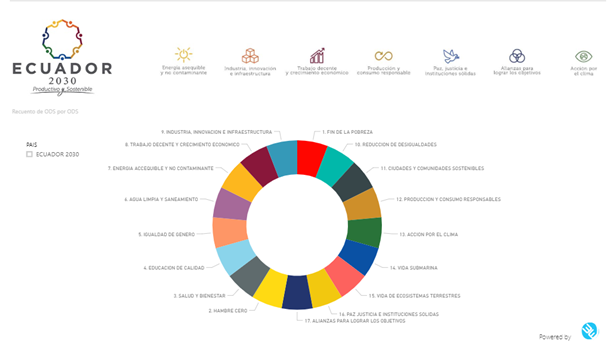
\includegraphics{objetivos.png}
    \caption{\label{Figura 1}{Objetivos de Desarrollo Sostenible, Ecuador}}
    %\label{fig:my_label}
\end{figure}


\section{Resultados}
\label{sec5} 
En la figura 2 se visualizan los tres principales ejes del Plan Nacional de desarrollo Toda una Vida, los cuales tienen en común el mejoramiento de la calidad de vida de las personas. A continuación se realiza una breve explicación de las opciones de uso de la inteligencia artificial para conseguir los propósitos planteados en cada eje.\\

\begin{figure}
    \centering
    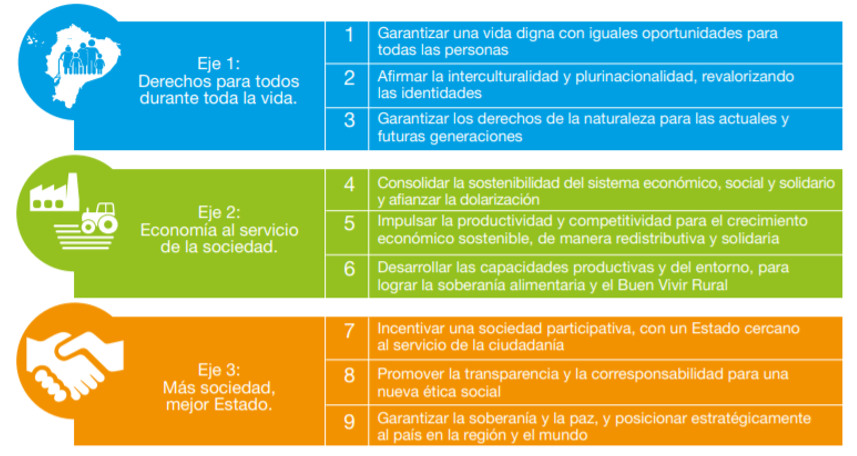
\includegraphics{toda una vida.png}
    \caption{\label{Figura 2}{Objetivos Nacionales de Desarrollol}}
    %\label{fig:my_label}
\end{figure}

\subsection{Eje 1: Derecho para todos durante toda una vida}
\label{subsec1}\\
Para ``garantizar una vida digna con iguales oportunidades para las personas", las aplicaciones médicas con el uso de redes neuronales en el reconocimiento de imágenes por computadora, la predicción en de posibles enfermedades o dolencias en el futuro de las personas con el uso de la clasificación supervisada de sus historias clínicas, el descubrimiento de nuevas cepas en virus que atacan a las personas con el uso de los algoritmos de uso genético, son algunos de los ejemplos de las posibilidades de aplicación de la inteligencia artificial para beneficio de la salud de las personas.\\

En cuanto a ``afirmar la interculturalidad y plurinacionalidad, revalorizando las identidades", se lograría con la aplicación de técnicas de clasificación supervisada para identificar aquellos aspectos de los pueblos y sus culturas que deben tener mayor atención en cuanto a apoyo para su desarrollo propio y evitar la migración. Un programa de diferentes actividades para fomentar el turismo y la conservación de la identidad de los pueblos, desenvocaría en el mantenimiento de la cultura, conocimientos y saberes ancestrales y actuales en el tiempo.\\

``Garantizar los derechos de la naturaleza para las actuales y futuras generaciones", la determinación de aquellos  peligros que asechan a la vida de la flora y la fauna marina, terrestre así como la silvestre en las selvas ecuatorianas, es una razón importante para mantener una constante vigilancia e identificación de los atentados contra la naturaleza. La implementación de dispositivos que identifiquen y notifiquen de manera urgente a las autoridades civiles y de socorro para evitar desastres ocasionados por el hombre así como desastres naturales producto de un mal mantenimiento del suelo y el ambiente, hacen de la inteligencia artificial un aliado de la conservación de la vida.\\


\subsection{Eje 2: Economía al servicio de la sociedad}
\label{subsec1}\\
``Consolidar la sostenibilidad del sistema económico, social y solidario y afianzar la dolarización", el constante mantenimiento y evaluación de los movimientos financieros en distintas instituciones gubernamentales como privadas, serán el soporte para la identificación de actividades fraudulentas, la evaluación de los algoritmos de machine learning y la identificación de valores anormales dan la pauta para su detección.\\

El control de las arcas financieras es más sencillo cuando es apoyado en procesos automatizados, la gran cantidad de información que se procesa al instante se convierte en el aliado de gerentes y propietarios de negocios, permitiendo su normal desarrollo y desembocando en un desarrollo general a nivel del país.\\

``Impulsar la productividad y competitividad para el crecimiento económico sostenible, de manera redistribuida y solidaria", el cálculo efectivo de distribución en planes y proyectos operativos se lograría si además del análisis finaciero se utilizara un análisis situacional basado en la realidad de las operaciones, es decir, mantener un recuento de las actividades y requerimientos que a diario se realizan con técnicas que utilicen el entrenamiento de redes neuronales para determinar de manera automática las prioridades de distribución económica, que permitan efectivamente desarrollar las actividades de crecimiento económico esperadas.\\

``Desarrollar las capacidades productivas y del entorno, para lograr la soberanía alimentaria y el Buen Vivir Rural", la educación y capacitación de talento humano es imprescindible. El desarrollo de los pueblos se palpa en la generación de empleos y desarrollo productivo. \\

Los diferentes problemas de educación vienen determinados por diferentes factores como: los recursos económico, el tiempo, la distancia, la tecnología. Es aquí donde la implementación de salones inteligentes, ubicados en zonas rurales, al alcance de las personas que necesitan capacitarse para mantener su productividad y conservación del suelo. Los conocimientos impartidos serían dependiendo de las necesidades y el tipo de producción. Por ejemplo si se necesitara de perfeccionamiento en el tratamiento de la leche, un tutor virtual pueda resolver las dudas y necesidades de información del usuario.\\

\subsection{Eje 3: Más sociedad mejor Estado}
\label{subsec1}\\
``Incentivar una sociedad participativa, con un estado cercano al servicio de la ciudadanía", Es precisamente la capacitación contínua de los habitantes lo que le llevan a desarrollar la innovación. La amplitud de conocimientos y la disponibilidad para desarrollar nuevas y variadas habilidades podrían ser resueltos de manera eficiente por robots inteligentes desarrollados específicamente para solventar las dudas en cuanto a conocimientos como a leyes y reglamentos. \\


``Promover la transparencia y la corresponsabilidad para una nueva ética social", las leyes de la robótica son claras, por cuanto se garantiza la vida de las personas a su alrededor. El desarrollo de planes, programas, leyes y reglamentos que formalicen en el conocimiento de los habitantes la importancia de mantener los datos personales en privado, así como respetar la información personal del resto de personas, promueven la cultura del cuidado de los datos personales tanto en medios virtuales como en documentos físicos.\\

La generación de nuevos modelos de detección de entidades, detección de sentimientos, detección de privacidad, entre otros, fortalecerán el cuidado de la información en el ámbito de dominio público de información.\\


``Garantizar la soberanía y la paz, y posicionar estratégicamente al país en la región y el mundo", la gobalización y la competitividad de los países hacen que se desarrollen las tecnologías que cubran los problemas y necesidades para afrontar la competencia.  El cuidado y protección de las fronteras por ejemplo, es clave para evitar desde la contamientación del suelo hasta la migración.\\

Los sistemas inteligentes que permitan un mejor control fronterizo es indiscutiblemente urgente en el país. La conexión con bases de datos internacionales para la identificación temprana de un posible atentado, por ejemplo, garantizan la paz. El reconocimiento facial, la identificación de documentos alterados o falsos son tareas que facilmente pueden ser resueltas por técnicas de procesamiento de imágenes y la percepción computacional.\\

En la figura 3 se explica la relación existente entre las necesidades de las tecnologías dotadas de inteligencia artificial y los sectores de desarrollo tecnológico que aportan a los diferentes tópicos de desarrollo de las naciones, identificándose el área del desarrollo sostenible como un área de beneficio de su uso.

\begin{figure}
    \centering
    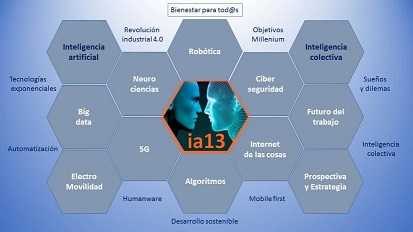
\includegraphics{lamina_panal_tematico_ia13.jpg}
    \caption{\label{Figura 3}{La inteligencia artificial para el desarrollo sostenible}}
    %\label{fig:my_label}
\end{figure}

\section{Conclusiones}
\label{sec6}
El progreso de los pueblos en gran medida se debe a la efectividad del uso de la tecnología, el desarrollo de nuevas inteligencias y procesamientos de información, permiten tomar mejores decisiones que promuevan la conservación de la vida en el tiempo.\\

La creación de nuevos modelos de clasificación automatizada de la información recolectada en cada una de las secretarias del país, permitirían solventar diferentes problemas de índole decisivo al momento de generar rubros económicos para la ejecución de obras de gran relevancia tanto de desarrollo como de sostenibilidad.\\

El desarrollo de nuevas carreras técnicas a nivel de país, que provean de talento humano especializado en el uso de los datos y generación de nuevos conocimientos con la aplicación de técnicas de inteligencia artificial, son necesarias y urgentes para lograr la consecución de los objetivos del gobierno en el corto plazo.




%% References
%%
%% Following citation commands can be used in the body text:
%% Usage of \cite is as follows:
%%   \cite{key}         ==>>  [#]
%%   \cite[chap. 2]{key} ==>> [#, chap. 2]
%%

%% References with bibTeX database:

\bibliographystyle{elsarticle-num}
% \bibliographystyle{elsarticle-harv}
% \bibliographystyle{elsarticle-num-names}
% \bibliographystyle{model1a-num-names}
% \bibliographystyle{model1b-num-names}
% \bibliographystyle{model1c-num-names}
% \bibliographystyle{model1-num-names}
% \bibliographystyle{model2-names}
% \bibliographystyle{model3a-num-names}
% \bibliographystyle{model3-num-names}
% \bibliographystyle{model4-names}
% \bibliographystyle{model5-names}
% \bibliographystyle{model6-num-names}

\bibliography{sample}


\end{document}

%%
%% End of file `elsarticle-template-num.tex'.
